%mark = star, diamond, square, otimes
%\documentclass{article}
%\usepackage{pgfplots}
%\usepackage[justification=centering]{caption}
%\pgfplotsset{compat=newest}
%\begin{document}
\begin{figure}[!h]
\centering

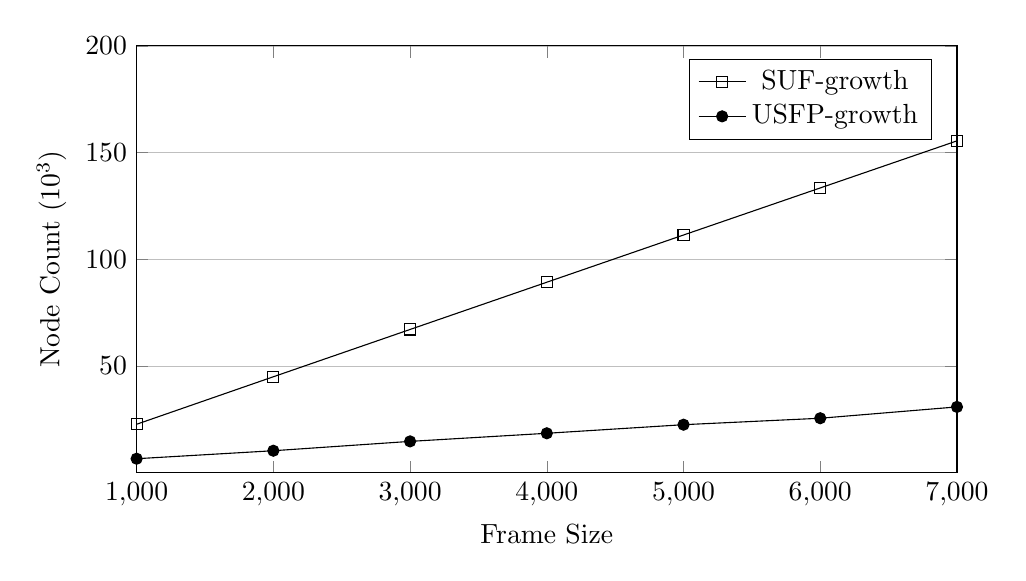
\begin{tikzpicture}
\begin{axis}[
 width=12cm,
   height=7cm,
    xlabel={Frame Size },
    ylabel={Node Count ($10^3$)},
    xmin=1000, xmax=7000,
    ymin=0, ymax=200,
    xtick={1000,2000,3000,4000,5000,6000,7000},
    ytick={50,100,150,200},
    legend pos=north east,
    ymajorgrids=true,
    grid style={line width=.2pt,draw=gray!50},
]
 
\addplot[
    solid, every mark/.append style={solid, fill=gray}, mark=square
    ]
    coordinates {
			(1000,22.597)
			(2000,44.862)
			(3000,67.033)
			(4000,89.175)
			(5000,111.313)
			(6000,133.377)
			(7000,155.435)



	};
    \addlegendentry{SUF-growth}
\addplot[
    solid, every mark/.append style={solid, fill=black}, mark=*
    ]
    coordinates {
			(1000,6.444)
			(2000,10.187)
			(3000,14.568)
			(4000,18.362)
			(5000,22.390)
			(6000,25.416)
			(7000,30.727)


};
    \addlegendentry{USFP-growth}
 
\end{axis}
\end{tikzpicture}
\caption{Total Tree Node vs Frame Size \\(Window Size = 2) for Mushroom database}
\label{result:mushroom_total_mem_node}
\end{figure}
%\end{document}